\documentclass[10pt]{article}

\usepackage[utf8]{inputenc}
\usepackage{floatrow}

\usepackage{algorithm, algpseudocode}
\let\oldReturn\Return
\renewcommand{\Return}{\State\oldReturn}
\newcommand{\N}{\mathbb{N}}
\newcommand{\R}{\mathbb{R}}
\usepackage[T1]{fontenc}
\usepackage{enumitem}
\usepackage{hyperref}
\usepackage{scrextend}
\usepackage{amsmath}
\usepackage{amsfonts}
\usepackage{stmaryrd}
\usepackage{graphicx}
\usepackage{color}
\usepackage{listings}
\usepackage{wrapfig}
\usepackage[hmargin=1.25in,vmargin=1.25in]{geometry}

%title setup
\title{Projet IPF: SUBSET-SUM-OPT}
\author{Romain PEREIRA}
\date{03/04/2018}

% table of contents setup
\renewcommand{\contentsname}{Sommaire}
\usepackage{etoolbox}
\patchcmd{\thebibliography}{\section*{\refname}}{}{}{}

\hypersetup{
    colorlinks,
    citecolor=black,
    filecolor=black,
    linkcolor=blue,
    urlcolor=red
}
			
\begin{document}
	\maketitle
	\tableofcontents

	\newpage
	\section{Préambule}

		Ce projet est réalisé dans le cadre de mes études à l'ENSIIE. Rappel de l'énoncé:
		\newline
		\begin{addmargin}[2em]{0em}
			\label{problem}{
			SUBSET-SUM-OPT - Etant donnée un ensemble fini $E$ d'entiers
			strictements positifs et un entier cible s, trouver l'entier
			$s' \leq s$ le plus grand possible, tel qu'il existe un
			sous-ensemble $E' \subseteq E$ vérifiant $\sum_{e \in E'}{e} = s'$.
			}
			\newline
		\end{addmargin}
		Ce rapport présente (en pseudo-code), les algorithmes implémentés.
		\newline
		Le code OCaml est disponible dans le rendu.
		\newline
		\subsection{Spécificités techniques}
			Un Makefile est disponible pour compiler le projet et les tests:
			\begin{itemize}[label=-]
				\setlength\itemsep{0.1em}
				\item \textit{make} : compile les fichiers sources avec les tests vers un executable \textbf{subset-sum-opt.out}
				\item \textit{clean} : supprimes les fichiers compilés temporaires (.mlo et .cmo)
				\item \textit{fclean} : supprimes tous les fichiers compilés (executable et temporaires)
			\end{itemize}
			Les testes sont unitaires et effectue dans l'ordre:
			\begin{itemize}[label=-]
				\item Les fonctions du module \textit{Listes}
				\item Les fonctions du module \textit{Ensembles}
				\item Les fonctions du module \textit{Approche\_naïve}
				\item Les fonctions du module \textit{Approche\_plus\_directe}
				\item Les fonctions du module \textit{Approche\_avec\_nettoyage}
				\item Les fonctions du module \textit{Approche\_diviser\_pour\_regner}
				\item Les fonctions du module \textit{Approche\_diviser\_pour\_regner}
				\item Comparaisons des approches
			\end{itemize}

		\subsection{Notations}
			J'utiliserai les notations suivantes:
			\begin{itemize}[label=-]
				\setlength\itemsep{0.1em}
				\item Soit $E$ est un ensemble, $Card(E)$ est le cardinal de $E$.
				\item Soit $E$ est un ensemble, $P(E)$ est l'ensemble formé des parties de $E$
			\end{itemize}
		\subsection{Rappels/Complexités}
			Soit $E$ un ensemble tel que $Card(E) = n$, alors
			$$Card(P(E)) = 2^n$$
			$$\forall E' \in P(E) , 0 <= Card(E') <= n$$
			\newpage
			On considèrera les complexités pour les opérations suivantes:
			\begin{itemize}[label=-]
				\setlength\itemsep{0.1em}
				\item Soit $(x, y)$ des scalaires, je considère que les 4 opérations élémentaires ($x+y$, $x-y$, $x*y$, $x/y$) sont en $O(1)$
				\item Soit 2 ensembles X, Y, $X \cup Y$ est une opération en $O(Card(X) * Card(Y))$
				\item Soit $E \subset \mathbb{N}$, $\max{E}$ est une opération en $O(Card(E))$
			\end{itemize}
			
			\subsection{Bonus}\label{bonus}
				L'implémentation a également été légèrement plus loin que les algorithmes présentés dans ce document: elle permet
				de savoir sur quelle partie $E' \subset E$ la somme $\sum\limits_{e \in E'}e = s$ a été atteinte.
				\newline
				\newline
				\textbf{La 1ère implémentation (qui est plus simple, mais sans l'ensemble sur lequel les sommes sont obtenus)
				est disponible dans le dossier 'bkp' du rendu.}

	\newpage
	\section{Approche naïve}\label{approche_naive}
		Cette approche consiste à determiner tous les sous-ensembles $E'$ de $E$, d'effectuer la somme sur
		tous les $E'$, et de renvoyer la somme la plus proche de $s$. Cette approche par 'force brute' est lourde.
		\subsection{Question 1 : somme sur un ensemble}
			\begin{algorithm}
				\caption{Renvoie la somme des éléments de E}
				\begin{algorithmic}[1]
					\Function{Somme}{$E' \subset \mathbb{N}$}
						\If{$E' = \emptyset$}
							\Return 0
						\EndIf
						\State Soit $x \in E'$
						\Return x + $\mathtt{Somme}(E' \backslash \{x\}$)
					\EndFunction
				\end{algorithmic}
			\end{algorithm}
			Complexité en $\boxed{O(n)}$, où $n = Card(E')$
			
		\subsection{Question 2 : génération des parties d'un ensemble}
			\begin{algorithm}
				\caption{Renvoie l'ensemble des parties de E}
				\begin{algorithmic}[1]
					\Function{Sous-ensembles}{$E \subset \mathbb{N}$}
						\If{$E = \emptyset$}
							\Return $\{\emptyset\}$
						\EndIf
						\State Soit $x \in E$
						\State Soit $P \leftarrow \mathtt{Sous-ensembles}(E \backslash \{x\})$
						\Return $P \cup \{E' \cup x \mid E' \in P\}$
					\EndFunction
				\end{algorithmic}
			\end{algorithm}
			Complexité en $\boxed{O(2^nn)}$, où $n = Card(E)$
		
		\subsection{Question 3 : résolution de SUBSET\_SUM\_OPT par force brute}
			\begin{algorithm}
				\caption{Renvoie la réponse au problème SUBSET\_SUM\_OPT sur (E, s)}
				\begin{algorithmic}[1]
					\Function{subset\_sum}{$E \subset \mathbb{N}, s \in \mathbb{N}$}
						\State Soit $P \leftarrow \mathtt{Sous-ensembles}(E)$
						\Return $\underset{E' \in P}{\max}\{s' \mid s' = \mathtt{Somme}(E') \quad et \quad s' \leq s\}$
					\EndFunction
				\end{algorithmic}
			\end{algorithm}
			Complexité en $\boxed{O(2^nn)}$, où $n = Card(E)$
			
	\newpage
	\section{Approche plus directe}\label{approche_plus_directe}
		Dans cette approche, plutot que de calculer l'ensemble des parties de $E$,
		on se propose de calculer l'ensemble des sommes atteignables en sommet sur les parties de $E$.
		
		\subsection{Question 4 : sommes atteignables}\label{get_all_sums}
			\begin{algorithm}
				\caption{Renvoie l'ensemble des entiers $s$ tels qu'il existe $E' \subseteq E$ vérifiant $\sum\limits_{e \in E'}e = s$}
				\begin{algorithmic}[1]
					\Function{get\_all\_sums}{$E \subset \mathbb{N}$}
						\If{$E = \emptyset$}
							\Return $\{0\}$
						\EndIf
						\State Soit $x \in E$
						\State $S \leftarrow \mathtt{get\_all\_sums}(E \backslash \{x\})$
						\Return $S \cup \{x + s \mid s \in S\}$
					\EndFunction
				\end{algorithmic}
			\end{algorithm}
			Si l'on suppose:
			\begin{itemize}[label=-]
				\setlength\itemsep{0.1em}
				\item $n = Card(E)$
				\item $m(n) = Card\{sommes \quad atteignables\} = \{s \mid \exists E' \subseteq E \mid \sum\limits_{e \in E'}e = s\} \leq 2^n$
			\end{itemize}
			Alors la complexité de cet algorithme est en $\boxed{O(m(n) * n)}$
			\begin{itemize}[label=-]
				\setlength\itemsep{0.1em}
				\item $n$ : nombre de récursion
				\item $m(n)$ : l'union
			\end{itemize}
			\textbf{Remarque:} Cette algorithme fourni les sommes atteignables dans un ordre croissant. ($\bullet < \bullet$)

		\subsection{Question 5 : résolution de SUBSET\_SUM\_OPT}
			Une fois l'ensemble des sommes atteignables calculés, la résolution du problème devient trivial.
			La complexité de cet algorithme de résolution est donc en $\boxed{O(m(n) * n)}$
			\begin{algorithm}
				\caption{Renvoie la réponse au problème SUBSET\_SUM\_OPT sur (E, s)}
				\begin{algorithmic}[1]
					\Function{subset\_sum}{$E \subset \mathbb{N}, s \in \mathbb{N}$}
						\State Soit $S \leftarrow \mathtt{get\_all\_sums}(E)$
						\Return $\max\{s' \in S \mid 0 \leq s' \leq s\}$
					\EndFunction
				\end{algorithmic}
			\end{algorithm}

	\newpage
	\section{Approche avec nettoyage}\label{approche_naive}
		On peut réduire la complexité de l'approche précèdente en réduisant ce que l'on a noté $m(n)$ (le nombre de sommes atteignables.
		Dans cette approche, on se propose d'ajouter un 'filtre' sur l'algorithme qui génère les sommes.
			\subsection{Question 6 ; fonction clean\_up}
				Le filtre (l'algorithme $\mathtt{clean\_up}$ est donnée dans l'énoncé. Cette fonction prends en paramètre:
				\begin{itemize}[label=-]
					\setlength\itemsep{0.1em}
					\item $E \subset \mathbb{N}$ : l'ensemble a filtré
					\item $s \in \mathbb{N}$ : un entier positif
					\item $\delta \in \mathbb{R}_+^*$ : un réel positif (généralement $\ll 1$)
				\end{itemize}
				Cette fonction renvoie un nouvel ensemble $E' \subset E$, tel que:
				\begin{itemize}[label=-]
					\setlength\itemsep{0.1em}
					\item	$\forall x \in E' , x \leq s$
					\item	Si l'on considère la suite croissante $(u_n)_{n \in \mathbb{N}}$ des éléments de $E'$,
							$\forall n \in \mathbb{N}, u_{n + 1} \geq (1 + \delta)u_n $.
				\end{itemize}
	
				Autrement dit, tous les entiers strictement supérieurs à $s$ sont supprimés, et 
				si l'on considère 2 entiers consécutifs de l'ensemble trié $x$ et $y$, tel que $x < y$,
				ils sont 'proches d'un rapport d'au moins $(1 + \delta)$, $y$ est supprimé.
				Ce filtre supprime donc les éléments de l'ensemble qui sont 'proches' l'un de l'autre (au regard de $\delta$).
				En supprimant des valeurs proches, on espère pouvoir former les mêmes sommes qu'avec toutes les valeurs,
				mais en effectuant ainsi moins de sommations.
				\newline
				\newline
				Par exemple, pour l'entrée $\llbracket 0, 100 \rrbracket$, $s = 90$ et $\delta=0.01$, on obtient la sortie
				$$[1; 2; 3; 4; 5; 6; 7; 8; 9; 10; 12; 14; 16; 18; 20; 23; 26; 29; 32; 36; 40; 45; 50; 56; 62; 69; 76; 84]$$
				On remarque que les valeurs les plus 'petites' sont convervés ($\leq 10$), et que plus les valeurs deviennent 'grandes',
				moins elles passent le filtre.
				

			\subsection{Question 7 : résolution de SUBSET\_SUM\_OPT}
				L'algorithme de résolution est également fourni dans l'énoncé.
				Il est le même que celui de 'l'approche plus directe' \ref{approche_plus_directe}, sauf que
				lors du calcul des sommes atteignables filtrés par la fonction $\mathtt{clean\_up}$.
				
				\begin{algorithm}
					\caption{Renvoie l'ensemble des entiers $s$ tels qu'il existe
							$E' \subseteq E$ vérifiant $\sum\limits_{e \in E'}e = s$, passant les tests du filtre}
					\begin{algorithmic}[1]
						\Function{get\_all\_sums\_2}{$E \subset \mathbb{N}$, $\delta \in \mathbb{R}^*_+$}
							\If{$E = \emptyset$}
								\Return $\{0\}$
							\EndIf
							\State Soit $x \in E$
							\State $S \leftarrow \mathtt{get\_all\_sums\_2}(E \backslash \{x\})$
							\Return $\mathtt{clean\_up}(S \cup \{x + s \mid s \in S\})$
						\EndFunction
					\end{algorithmic}
				\end{algorithm}
			
			\begin{algorithm}
				\caption{Renvoie la réponse au problème SUBSET\_SUM\_OPT sur (E, s)}
				\begin{algorithmic}[1]
					\Function{subset\_sum}{$E \subset \mathbb{N}, s \in \mathbb{N}$}
						\State Soit $S \leftarrow \mathtt{get\_all\_sums\_2}(E, \delta)$
						\Return $\max\{s' \in S \mid 0 \leq s' \leq s\}$
					\EndFunction
				\end{algorithmic}
			\end{algorithm}
			La complexité de cet algorithme de résolution est donc en $\boxed{O(m'(n) * n)}$,
			avec $$m'(n) = Card\{sommes \quad atteignables \quad filtres\} \leq m(n) \leq 2^n$$.
			\textbf{Attention} cependant, pour $\delta$ trop grand, on perd l'optimalité du résultat.

		\newpage
		\section{Approche de type \textit{Diviser pour régner}}\label{approche_diviser_pour_regner}
			\subsection{Question 8 : is\_feasible}\label{is_feasible}
				On nous demande ici de créer une fonction qui sur la donnée d'un entier $s$, d'une liste $l_1$ d'entier croissant,
				d'une liste $l_2$ d'entier décroissant, renvoie $true$ si $s$ s'écrit comme la somme d'un élément de $l_1$ et d'un
				élément de $l_2$, et $false$ sinon.
				\newline
				La fonction implémenté suit l'algorithme suivant, qui se sert au maximum du fait que les listes soit triés.
				Les 3 cas de retours possibles sont:
				
				\begin{itemize}[label=-]
					\setlength\itemsep{0.1em}
					\item $\mathtt{TOO\_SMALL}$ : Soit $y \in l_2$, $\forall x \in l1, x + y < s \Rightarrow \forall y' < y, x + y' < x + y < s$.
					En français, pour $y$ fixer, la somme des $x + y$ avec $x$ dans $l_1$ est toujours inférieur à $s$.
					Pour un $y$ plus petit, on ne risque donc pas d'atteindre une valeur plus proche de $s$.
					\item $\mathtt{REACHED}$ : on a réussi à atteindre $s$.
					\item $\mathtt{TOO\_BIG}$ : On a parcouru toutes les valeurs de $l_2$, pour toutes les valeurs de $l_1$,
					sans avoir pu obtenir de couple $(x, y) \in l_1 \times l_2$ tel que $x + y <= s$.
				\end{itemize}
				
				\begin{algorithm}
					\caption{Renvoie \textbf{true} si $\exists (x, y) \in l_1 \times l_2 \mid x + y = s$, \textbf{faux} sinon}
					\begin{algorithmic}[1]
						\Function{is\_feasible}{$s \in \mathbb{N}$,
												$l_1 \subset \mathbb{N}$,
												$l_2 \subset \mathbb{N}$}
							\For{$y \in l_2$ (pris du plus grand au plus petit)}
								\For{$x \in l_1$ (pris du plus petit au plus grand)}
									\If{$x + y = s$}
										\State \textbf{Renvoyer true} (cas $\mathtt{REACHED}$)
									\ElsIf{$x + y > s$}
										\State \textbf{Passer au $y$ suivant} (cas $\mathtt{TOO\_BIG}$)
									\Else (si $x + y < s$)
										\State \textbf{Passer au $x$ suivant} (car $x + y$ est déjà plus petit que 's')
									\EndIf
								\EndFor
								\State \textbf{Renvoyer faux} (cas $\mathtt{TOO\_SMALL}$)
							\EndFor
							\State \textbf{Renvoyer faux} (on a eu que des cas $\mathtt{TOO\_BIG}$)
						\EndFunction
					\end{algorithmic}
				\end{algorithm}
				
				Les complexités sont:
				\begin{itemize}[label=-]
					\setlength\itemsep{0.1em}
					\item Dans le pire des cas (où l'on a que des cas $TOO_BIG$) : $O(Card(l_1)Card(l_2)$
					\item Dans le meilleur des cas (cas $REACHED$ avec le 1er $y$ et le 1er $x$...) : $O(1)$ (peu probable)
					\item Le cas moyen n'est pas évident à évaluer, étant donné que $l_1$ et $l_2$ dépendent de nombreux paramètres...
				\end{itemize}

			\subsection{Question 9 : best\_feasible}\label{best_feasible}
				Au regard de la Question 8 (\ref{is_feasible}), on nous demande maintenant de créer une fonction qui sur
				la donnée d'un entier $s$, d'une liste $l_1$ d'entier croissant, d'une liste $l_2$ d'entier décroissant,
				renvoie le plus grand entier $s' \leq s$ somme d'un élément de $l_1$ et d'un élément de $l_2$
				\newline
				\newline
				N.B: non explicitement dis dans le sujet, mais si un tel entier $s'$ n'existe pas, $-1$ est renvoyé.
				\begin{algorithm}
					\caption{Renvoie $\underset{(x, y) \in l_1 \times l_2}{\max}\{x + y \mid x + y < s\}$}
					\begin{algorithmic}[1]
						\Function{best\_feasible}{$s \in \mathbb{N}$,
												$l_1 \subset \mathbb{N}$,
												$l_2 \subset \mathbb{N}$}
							\State $s' \leftarrow -1$
							\For{$y \in l_2$ (pris du plus grand au plus petit)}
								\For{$x \in l_1$ (pris du plus petit au plus grand)}
									\If{$x + y = s$}
										\State \textbf{Renvoyer $s$} (cas $\mathtt{REACHED}$)
									\ElsIf{$x + y > s$}
										\State \textbf{Passer au $y$ suivant} (cas $\mathtt{TOO\_BIG}$)
									\Else (si $x + y < s$)
										\If{$x + y > s'$}
											\State $s' \leftarrow x + y$
										\EndIf
										\State \textbf{Passer au $x$ suivant}
									\EndIf
								\EndFor
								\State \textbf{Renvoyer $s'$} (cas $\mathtt{TOO\_SMALL}$).
							\EndFor
							\State \textbf{Renvoyer $s'$} (on a eu que des cas $\mathtt{TOO\_BIG}$)
						\EndFunction
					\end{algorithmic}
				\end{algorithm}
				
			\subsection{Question 10 : résolution de SUBSET\_SUM\_OPT}
				En se servant des fonctions \ref{get_all_sums}, \ref{best_feasible},
				en en ajoutant 2 fonctions subsidiaires (voir \textit{Listes.ml})
				\begin{itemize}[label=-]
					\setlength\itemsep{0.1em}
					\item $\mathtt{split}$ : sépares une liste en 2 sous liste de longueur égal (à 1 prêt)
					\item $\mathtt{sort}$ : tri les éléments dans l'ordre croissant
					\item $\mathtt{invsort}$ : tri les éléments dans l'ordre décroissant
				\end{itemize}
				on peut élaborer l'algorithme de résolution suivant, qui se base sur l'idée de 'diviser pour régner':
				\begin{algorithm}
					\caption{Renvoie la réponse au problème SUBSET\_SUM\_OPT sur (E, s)}
					\begin{algorithmic}[1]
						\Function{subset\_sum}{$E \subset \mathbb{N}, s \in \mathbb{N}$}
							\State $(l_1, l_2) \leftarrow \mathtt{split}(l)$
							\State $(s_1, s_2) \leftarrow (\mathtt{get\_all\_sums}(l1), \mathtt{get\_all\_sums}(l2))$
							\Return $\mathtt{best\_feasible}(s, \mathtt{sort}(s_1), \mathtt{invsort}(s_2))$
						\EndFunction
					\end{algorithmic}
				\end{algorithm}
				
		\section{Comparaison des approches et améliorations}
			\subsection{Question 11}
				(voir 'tests.ml')
			\subsection{Question 12}
				(voir 'tests.ml')
			\subsection{Question 13 : Bonus}
				Comme dit précèdemment (\ref{bonus}), ce bonus a été effectué: les fonctions de résolution renvoie également
				le sous-ensemble sur lequel la somme a été obtenu.

			\subsection{Illustration}\label{illustrations}
			
				Les graphiques suivants ont été généré sur les tests suivant:
				\begin{itemize}[label=-]
					\setlength\itemsep{0.1em}
					\item 1) Fixer $n = Card(E)$
					\item 2) Générer un ensemble $E \subset \mathbb{N}$ tel que $Card(E) = n$ et $\forall x \in E, 1 \leq x \leq 2n$
					\item 3) Résoudre le probleme: $SUBSET\_SUM(s = \frac{n * \frac{n}{2}}{2}, E)$ avec les 4 approches.
				\end{itemize}
				
				Pour $1 \leq n \leq 17$, toutes les résolutions fonctionnent, et on obtient ces allures de courbes:
				
				\begin{figure}[H]
					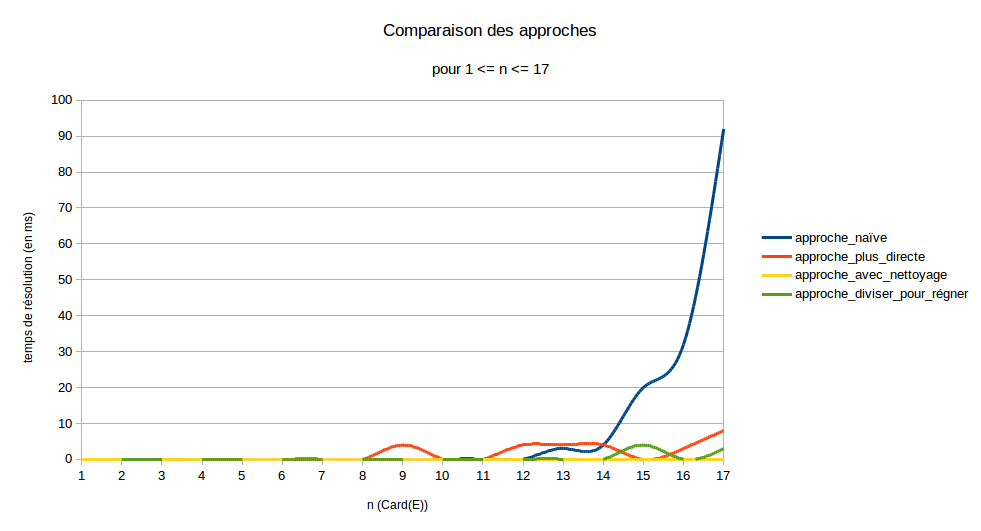
\includegraphics[width=16cm]{./images/cmp_n_1_17.png}
					\caption{\textit{La complexité de l'approche naïve suit effectivement une allure exponentielle}}
				\end{figure}

				\newpage
				Pour $n > 18$, l'approche naïve (\ref{approche_naive}) provoque une erreur de dépassement de pile, je n'ai pas pu
				la tester pour des $n$ plus grands.
				\begin{figure}[H]
					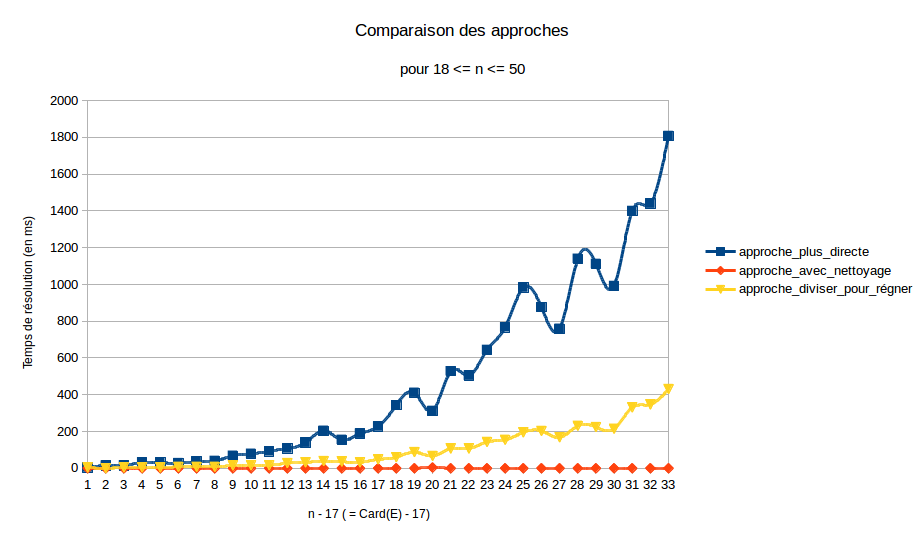
\includegraphics[width=16cm]{./images/cmp_n_18_50.png}
				\end{figure}
				On remarque que l'approche plus directe (\ref{approche_plus_directe}) a une allure exponentielle (en $O(2^n)$),
				et que l'approche 'diviser pour régner' (\ref{approche_diviser_pour_regner}) aussi, mais avec une allure plus 'écrasé'.
				
				\newpage
				Pour $n \geq 50$, l'approche diviser pour régner prends plus de 2 secondes... Voici les performances de l'approche avec nettoyage
				pour $n \gg 1$:
				\begin{figure}[H]
					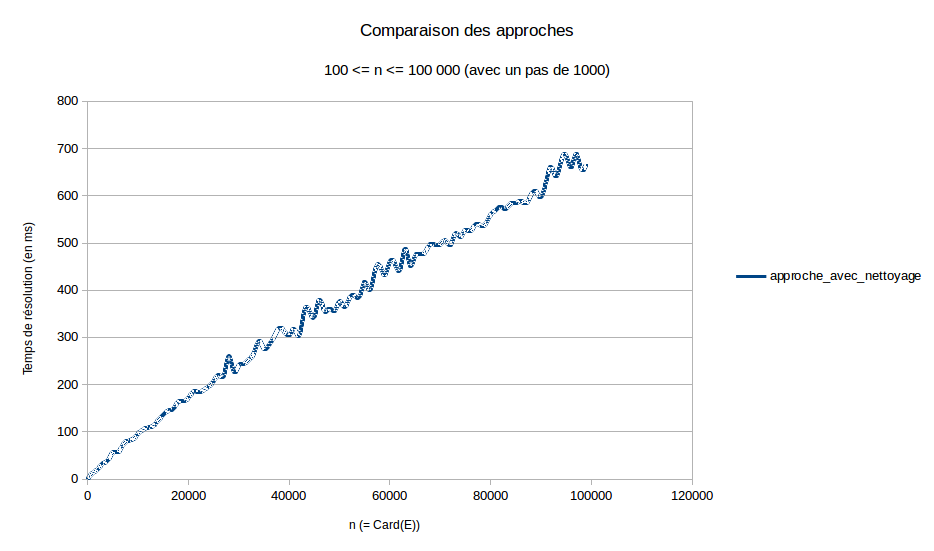
\includegraphics[width=18cm]{./images/approche_avec_nettoyage_100_1000_100000.png}
				\end{figure}
				Pour $n \geq 140\quad000$, j'obtiens un dépassement de pile sur ma machine.
				\newline
				Les résultats ont été obtenus pour $\delta = 10^{-7}$, et si l'on note $r$ le résultat obtenu,
				il s'éloigne d'au plus $1\%$ de $s$ $$100 \frac{r}{s} \leq 0.01$$
				\newline
				\newline
				\textbf{N.B:} Les données brutes (format .csv) sont disponibles dans le rendu.
		\newpage
		\section{Conclusion}
			L'objectif de ce projet était de résoudre le problème SUBSET\_SUM\_OPT \ref{problem}, problème NP-difficle,
			à l'aide de différentes approches, puis de comparer les résultats obtenus.
			\newline
			\newline
			L'implémentation des 4 méthodes demandées a été effectué avec succès.
			\newline
			
			Pour les méthodes naïve, plus directe, et de type diviser pour régner, le résultat obtenu est optimal.
			Bien que ces algorithmes soient plus longs que l'approche avec nettoyage, on s'assure l'optimalité du résultat
			et donc la réponse au problème.
			\newline
			Cependant, pour des valeurs de $n = Card(E)$ trop grandes ($ > 50$), nos implémentations sont lentes ($\geq 4 sec.)$,
			ou pire, elles atteignent les limites de la machine et s'arrête suite à des dépassements de piles.
			\newline
			
			L'approche avec nettoyage quant à elle est plus rapide (voir Illustrations \ref{illustrations}),
			mais ne permet de trouver une solution optimal.
			\newline
			\newline
			Pour aller plus loin dans la résolution du problème, il est donc maintenant question de savoir
			s'il existe des structures de données permettant d'optimiser nos algorithmes
			(l'utilisation d'une pile explicit en mémoire RAM, au lieu de la pile-machine pour éviter les dépassements de pile, par exemple),
			ou bien encore d'autres algorithmes plus performant donnant une solution exacte (nottement en allant plus loin dans la logique
			de 'diviser pour régner', ou en trouvant un filtre type 'clean\_up' qui garanti tout de même l'optimalité)
			\newline
			\newline
			Quelques recherches ont été effectué sur ces pistes, mais n'ont pas pu être mis en oeuvre par manque de temps.
			
	\newpage
	\section{Références}
		\begin{thebibliography}{}
			\bibitem{ocaml}
				'Module List' - INRIA\newline
				\href{https://caml.inria.fr/pub/docs/manual-ocaml/libref/List.html}
				      {\textit{https://caml.inria.fr/pub/docs/manual-ocaml/libref/List.html}}
				      
			\bibitem{sous_ensembles}
				'Ensemble des parties d'un ensemble' - Wikipédia\newline
				\href{https://fr.wikipedia.org/wiki/Ensemble\_des\_parties\_d'un\_ensemble}
				      {\textit{https://fr.wikipedia.org/wiki/Ensemble\_des\_parties\_d'un\_ensemble}}
				      
  \end{thebibliography}

\end{document}
